\documentclass[10pt]{beamer}

\usetheme[progressbar=frametitle]{metropolis}

\usepackage{appendixnumberbeamer}

\usepackage{booktabs}
\usepackage[scale=2]{ccicons}

\usepackage{pgfplots}
\usepgfplotslibrary{dateplot}
\usepackage{subfig}

\usepackage{xspace}
\newcommand{\themename}{\textbf{\textsc{metropolis}}\xspace}

%% drawings
\usepackage{tikz}
\usetikzlibrary{quantikz}

%% per final smile
\usepackage{fontawesome}

% align images to bullets
\usepackage{adjustbox}

\title{A Glimpse into Quantum-enhanced Machine Learning Solutions}

\date{April 27, 2022}
%\date{\today}

\author{
	Massimiliano Pronesti, 
	Federico Tiblias, 
	Giulio Corallo
}

\institute{Amadeus Knowledge Sharing Session}


\begin{document}
	
	\maketitle
	
	% "who are we" slide
	\begin{frame}{Who are we?}

Three Computer Engineering and Data Science students interested in Machine Learning and fascinated by Quantum Computing
    
\end{frame}


	
	% outline
	\begin{frame}{Outline}
		\setbeamertemplate{section in toc}[sections numbered]
		\tableofcontents
		%[hideallsubsections]
		% uncomment the above line to hide subsections
	\end{frame}
	
	% actual content
	% path for images
\graphicspath{{assets/motivation/}}

\section[Motivation]{Motivation}

%%
\begin{frame}{Why going Quantum ?}
	Until now, we’ve relied on supercomputers to solve most problems. These are very large classical computers, often with thousands of classical CPU and GPU cores. However, supercomputers are not very good at solving certain types of problems, which seem easy at first glance. 
	\begin{center}
	    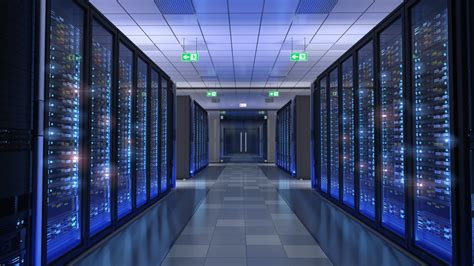
\includegraphics[width=.7\linewidth]{supercomputer}
	\end{center}
\end{frame}

%%
\begin{frame}{Why going Quantum ? A simple example}
	
Imagine you want to seat 10 fussy people at a dinner party, where there is only one optimal seating plan out of all the different possible combinations. How many different combinations would you have to explore to find the optimal?

Can you guess how many \alert{combinations}\footnote{Example from IBM's website \url{https://www.ibm.com/quantum-computing/what-is-quantum-computing/}} ?
\end{frame}


%% animation
\begin{frame}[<+- | only+>]{Why going Quantum ? A simple example}
	\metroset{block=fill}
	
	
	\begin{exampleblock}{For 2 people}
		2 Total combinations.
	\end{exampleblock}

	\begin{block}{For 5 people}
		120 Total combinations.
	\end{block}
	

	\begin{alertblock}{For 10 people}
		Over 3 Million of total combinations!!!
	\end{alertblock}	
	
	\begin{itemize}
		\item Supercomputers don't have the working \alert{memory} to hold the myriad combinations of real world problems.
		\item Supercomputers have to analyze each combination one after another, which can take a long \alert{time}.
	\end{itemize}
\end{frame}

\begin{frame}{Why going Quantum?}
\begin{figure}[H]
    \centering
    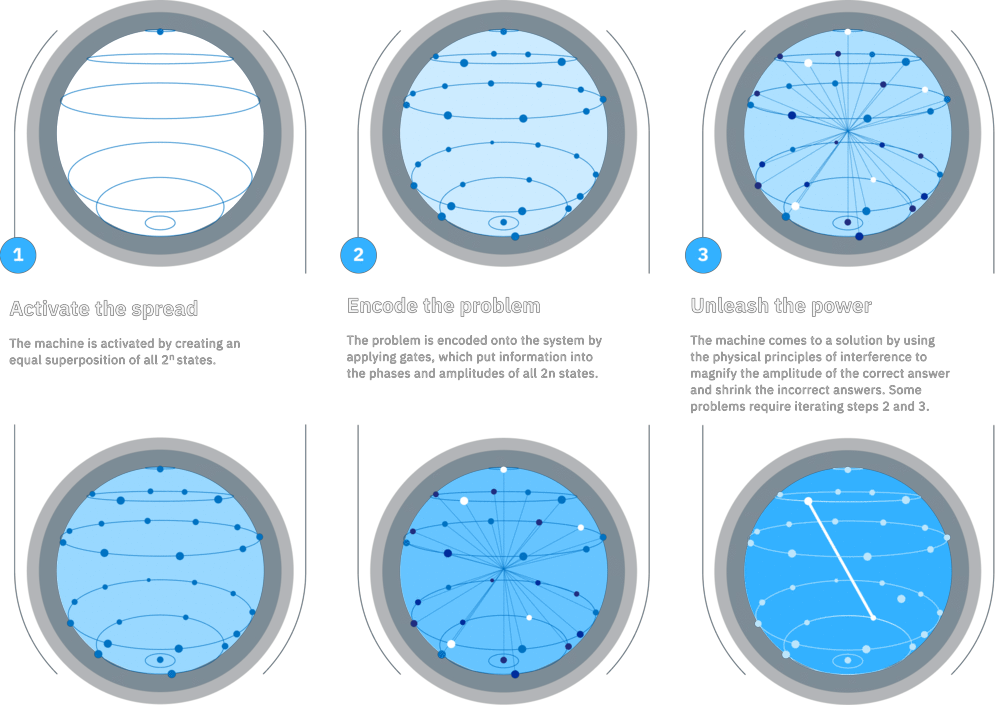
\includegraphics[width=.7\linewidth]{ quantumsup.png}
    \caption{Quantum Supremacy}
\end{figure}
\begin{itemize}
    \item Quantum computers can create vast multidimensional spaces in which to represent these very large problems. Classical supercomputers cannot do this.
   
\end{itemize}
  
\end{frame}

\begin{frame}{Why going Quantum ?}
\begin{itemize}
 \item Referring to the "10 fussy people at a dinner party" problem, with \alert{22 qubit} we can represent $2^{22} = 4194304$ states.
    \item The computation may be carried out on all those numbers in a \alert{single parallel computation}. This built-in parallelism is the key to the power of quantum computers.
\end{itemize}
    
\end{frame}


%%
\begin{frame}{How is a Quantum computer programmed?}
\begin{figure}[H]
    \centering
    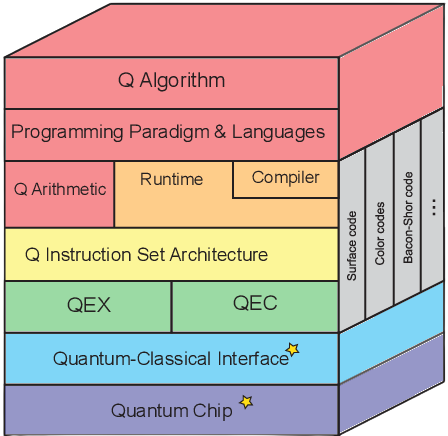
\includegraphics[width=.4\linewidth]{ Hto8a.png}
    \caption{Quantum Computer Architecture}
\end{figure}
There is an \alert{interface} between quantum mechanical processes and classical computer processes. Through this interface, input data from a a classical computing device can be fed into a quantum circuit.
\end{frame}

%%
\begin{frame}{How is a Quantum computer programmed?}
    \begin{itemize}
        \item \alert{Quantum Circuits} are constructed from Quantum Registers.
        \item \alert{Quantum Register} is a type of circuit construction from logical qubits. 
        \item \alert{Logical Qubits} can create different permutations and combinations of physical qubit manifestations.
    \end{itemize}
\end{frame}

%%
\begin{frame}[fragile]{What are Quantum Computers good at ?}
    \begin{figure}[!htb]
        \subfloat[Linear Algebra]{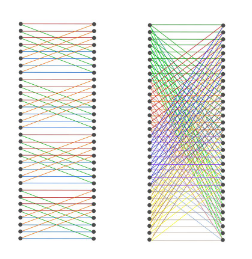
\includegraphics[width=0.3\linewidth]{linalg}} \quad
		 \subfloat[Sampling]{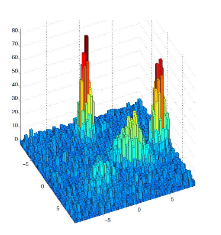
\includegraphics[width=0.3\linewidth]{sampling}} \quad
		 \subfloat[Optimization]{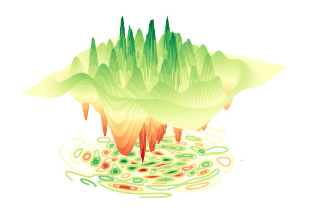
\includegraphics[width=0.33\linewidth, height=0.38\textheight]{optimiz}} 
    \end{figure}
    %
	%cose da dire: 
	%\begin{itemize}
	%	\item Linear Algebra
	%	\item Optimization
	%	\item Sampling
	%	\item Research Algorithms
	%\end{itemize}
\end{frame}


%%
\begin{frame}[fragile]{A Growing Interest in the field}
	cose da dire: 
	\begin{itemize}
	 \item tanti framework (qiskit, pennylane, cirq, tensorflow quantum, ...)
	 \item  tanti paperi (con plot della crescita 2012-2021)
	 \item  tutti (Microsoft, Google, IBM, NVidia ... ) hanno/vogliono un computer quantistico
	 \item  tanta ricerca nel settore Quantum Programming Languages
	\end{itemize}
\end{frame}    
    % path for images
\graphicspath{{assets/foundations/}}

\section[Quantum Computing Foundations]{Quantum Computing Foundations}

\begin{frame}{Bra-ket notation}
    Useful for representing quantum systems
		\begin{columns}[T,onlytextwidth]
			\column{0.5\textwidth}
			\centering
			Bra $=$ Row
			\begin{align*}
			    \langle A\rvert
			     = 
                \begin{bmatrix}
                a_{0} & a_{1} & a_{2} & \cdots
                \end{bmatrix}
            \end{align*}
			\column{0.5\textwidth}
			\centering
			Ket $=$ Column
            \begin{align*}
			    \lvert B\rangle
			     = 
                \begin{bmatrix}
                b_{0} \\
                b_{1} \\
                b_{2} \\
                \vdots \\
                \end{bmatrix}
            \end{align*}
		\end{columns}
		Properties \& operations:
		\begin{itemize}
			\item Scalar product $= \langle A\lvert B \rangle = [a_{0}, a_{1}, a_{2}, \cdots] \cdot [b_{0}, b_{1}, b_{2}, \cdots]^T$ 
			\item Norm $= \langle A\lvert A \rangle = |A|^2$
		\end{itemize}
    
\end{frame}

\begin{frame}{What is a qubit?}

		\begin{itemize}
			\item Building block for quantum computers
			\item 2-state quantum system (photon, electron, Schrödinger's cat, ...)
			\item 0, 1, both at the same time (superposition)
			\item Can be manipulated (quantum circuits)
			\item Can form more complex quantum systems (multi-quibit systems)
			\item Can be observed causing its collapse (measurement)
		\end{itemize}
		
		\begin{figure}[H]
          \centering
            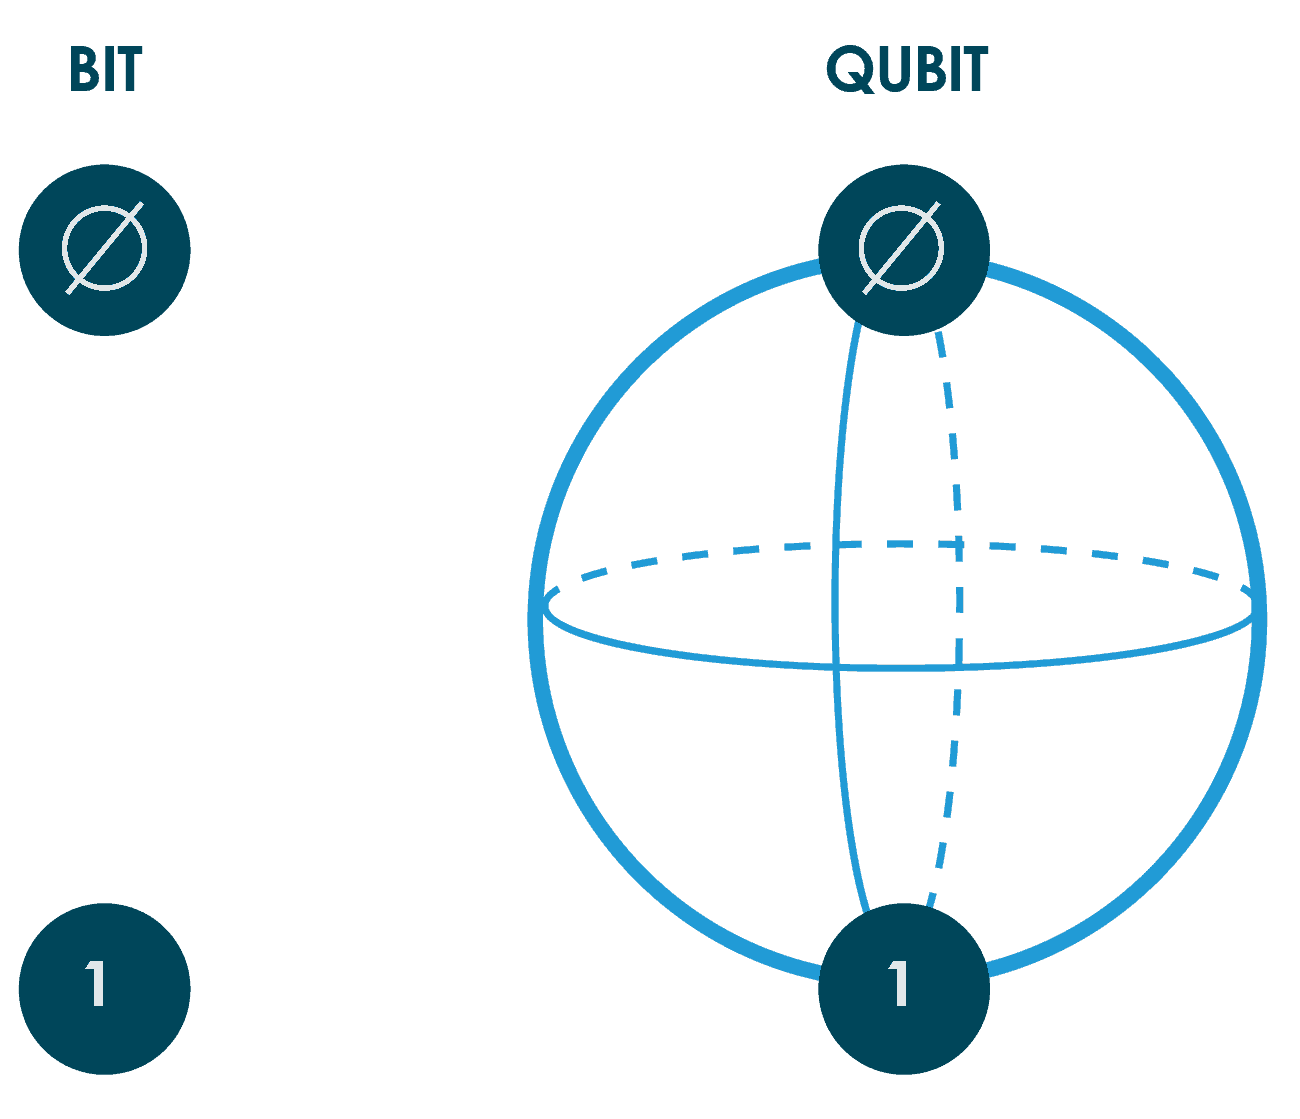
\includegraphics[width=.4\linewidth]{qubit}
        \end{figure}
    
\end{frame}

\begin{frame}{What is a qubit?}
		\begin{itemize}
			\item What does it mean to be 0 and 1 simultaneously?
			
			    It's a matter of probability during measurement
			
            \item Bra-ket qubit representation:
            \begin{columns}[T,onlytextwidth]
			\column{0.33\textwidth}
			\centering
			\begin{align*}
			    \lvert 0\rangle
			     = 
                \begin{bmatrix}
                1 \\
                0
                \end{bmatrix}
            \end{align*}
			
			\column{0.33\textwidth}
			\centering
            \begin{align*}
			    \lvert 1\rangle
			    = 
                \begin{bmatrix}
                0 \\
                1
                \end{bmatrix}
            \end{align*}
            
            \column{0.33\textwidth}
			\centering
            \begin{align*}
			    \lvert \psi\rangle
			    = 
                \begin{bmatrix}
                \psi_0 \\
                \psi_1
                \end{bmatrix}
            \end{align*}
		\end{columns}
		
		
		\item Probability measurement:
		    \begin{align*}
			    P(\lvert \psi\rangle = 0) = \lvert\psi_0\rvert^2
			\end{align*}
			\begin{align*}
			    P(\lvert \psi\rangle = 1) = \lvert\psi_1\rvert^2
            \end{align*}
		\item Probability distribution: $\langle \psi\lvert \psi \rangle = |\psi|^2 = 1 \ \forall \ \psi$

        \end{itemize}
\end{frame}

\begin{frame}{Multi-qubit system and entanglement}
    How can we represent 2 or more qubits with bra-kets? 
    
    With tensor products and longer vectors
    \begin{align*}
	    \lvert AB\rangle
		=
		\begin{bmatrix}
        a_0 \\       
        a_1 \\
        \end{bmatrix}
		\otimes
        \begin{bmatrix}
        b_0 \\       
        b_1 \\
        \end{bmatrix}
        =
        \begin{bmatrix}
        a_0 b_0 \\
        a_0 b_1 \\
        a_1 b_0 \\
        a_1 b_1 \\
        \end{bmatrix}
    \end{align*}
    By stacking $n$ qubits we can represent $2^n$ infinite precision numbers
    
    \centering
    $P(A = 0, B = 1) = \lvert a_0 b_1 \rvert^2 $
\end{frame}


\begin{frame}{Multi-qubit system and entanglement}
    How can we represent state $\lvert 00\rangle + \lvert 11\rangle $ with a tensor product? 
    
    We can't as there is no set of values for $a_0, a_1, b_0, b_1$ that allows it.
    \begin{align*}
	    \lvert AB\rangle
		=
		\begin{bmatrix}
        a_0 b_0 \\
        a_0 b_1 \\
        a_1 b_0 \\
        a_1 b_1 \\
        \end{bmatrix}
    \end{align*}
    
    However, we can still create this state with quantum circuits. The resulting state is said to be entangled as measuring one qubit immediately tells us the state of the other.
    \begin{align*}
	    \lvert 00\rangle + \lvert 11\rangle 
		=
		\begin{bmatrix}
        1/\sqrt{2} \\
        0 \\
        0 \\
        1/\sqrt{2} \\
        \end{bmatrix}
    \end{align*}
\end{frame}

	% path for images
\graphicspath{{assets/qml/}}

\section[Quantum Machine Learning]{Quantum Machine Learning}

%%
\begin{frame}{How can ML benefit from Quantum Computers ? }
	\begin{itemize}
		\item AI/ML already uses (massively) special-purpose processors: GPUs, TPUs, ASICs
		\item  Quantum computers (\alert{QPUs}) could be used as special-purpose AI
		accelerators
		\item May enable training of \alert{previously intractable} models
	\end{itemize}
\begin{figure}[H]
	\centering
	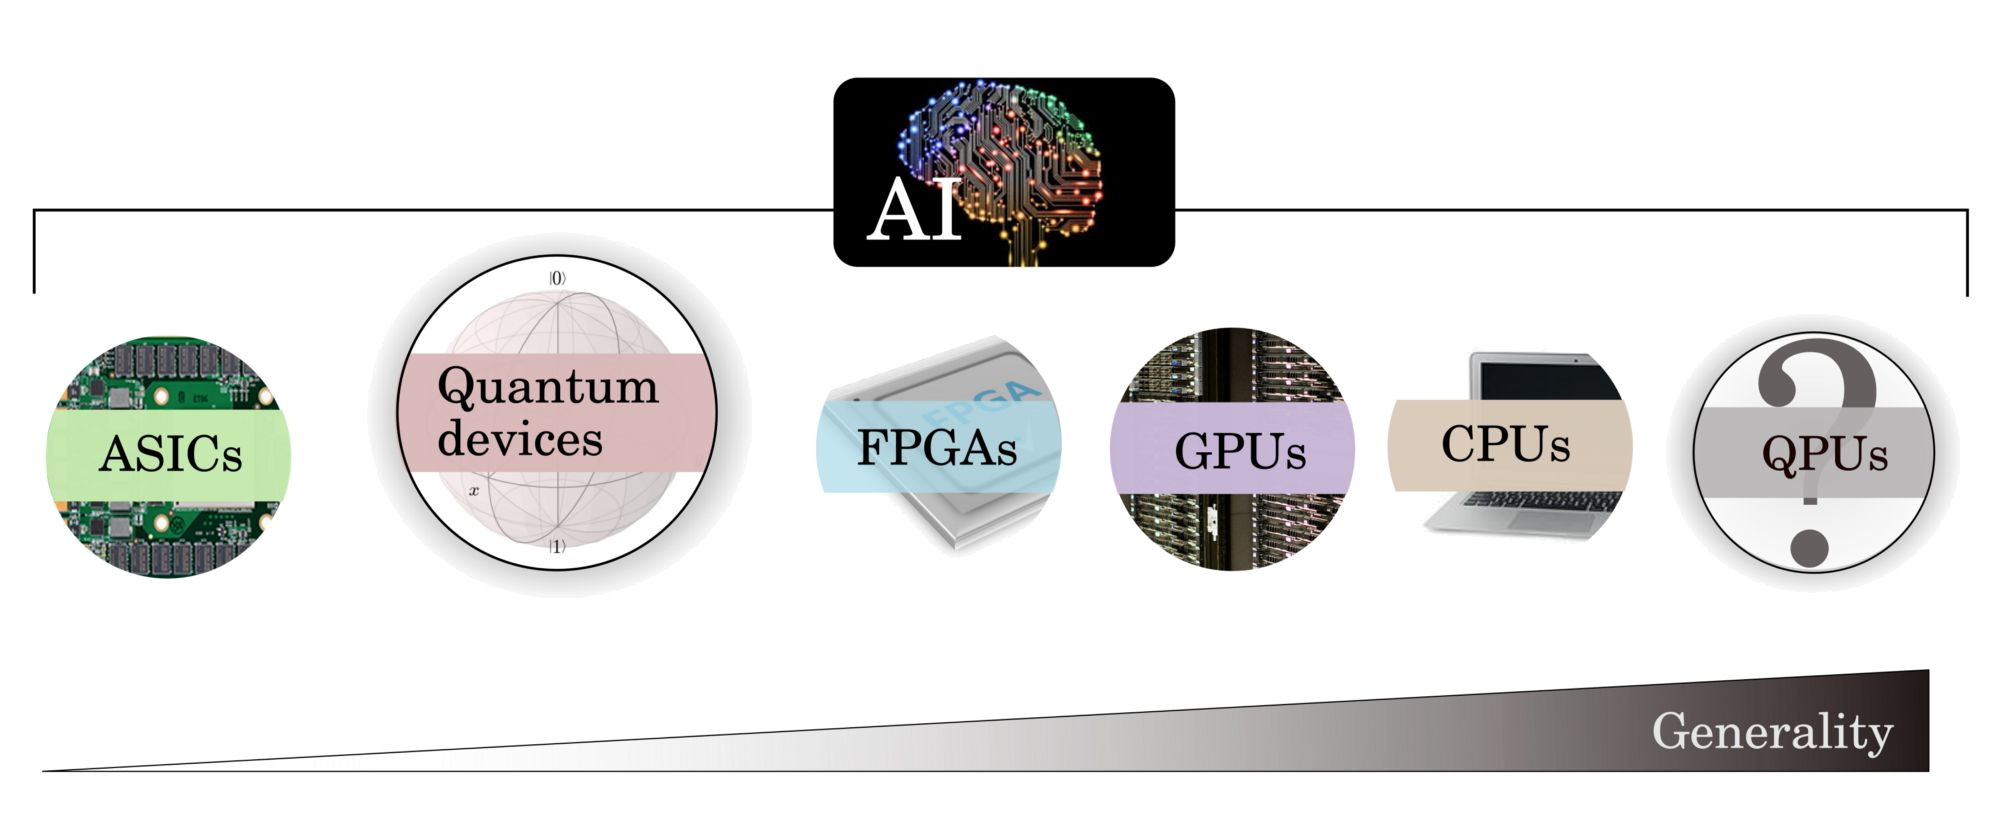
\includegraphics[width=.7\linewidth]{ qpu}
\end{figure}
\end{frame}

%%
\begin{frame}{How can ML benefit from Quantum Computers? }
	Quantum computing can also lead to \alert{new} machine learning models\\
	Examples currently being studied are:
	 \begin{itemize}
	 	\item \alert{Tensor Networks}
	 	\item Kernel methods
	 	\item Boltzmann machines
	 	\item \alert{Variational Quantum Circuits}
	 	\item Quantum Neural Networks
	 \end{itemize}
	\small
	\centering
 	\begin{quantikz}
    	& \gate[wires=3][2cm]{\mathcal{U}_1(\theta_1, \phi_1)}& \gate{S(r_1)} & \gate[wires=3][2cm]{\mathcal{U}_2(\theta_2, \phi_2)} & \gate{D(\alpha_1)} & \gate{\Phi(\lambda_1)}  & \qw\\
    	&  & \vdots \ \ \ & \vdots & \vdots & \vdots  \\ 
    	& \qw 										& \gate{\mathcal{S}(r_N)} & \qw  & \gate{\mathcal{D}(\alpha_N)} & \gate{\Phi(\lambda_N)} & \qw
    \end{quantikz}
\end{frame}

%%
\begin{frame}{A lesson from Deep Learning's success}
	\begin{Large}
		Why is Deep Learning \alert{Successful} ? 
	\end{Large}

	\begin{itemize}
		\item hardware advancements(GPUs, recently TPUs)
		\item Workhorse algorithms (backprop, stochastic GD, ...)
		\item specialized, user-friendly, maintained, high-perfomance software (PyTorch, Tensorflow, Keras)
		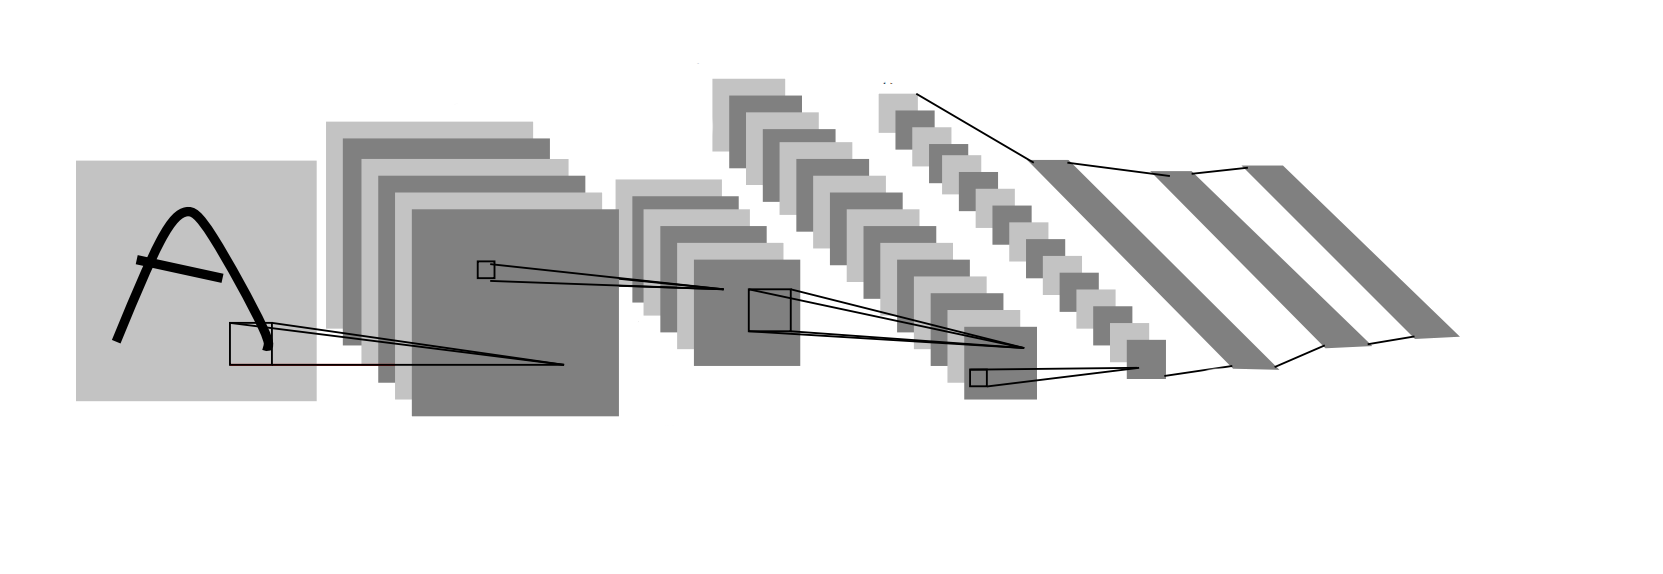
\includegraphics[width=\linewidth]{lenet-5}
	\end{itemize}	
\end{frame}

%%
\begin{frame}{What can we leverage?}
	\begin{itemize}
		\item hardware advancements(GPUs, TPUs + \alert{QPUs})
		\item 
		workhorse algorithms\\ (\alert{quantum-aware} backpropagation, stochastic GD, ...)
		\begin{center}
		  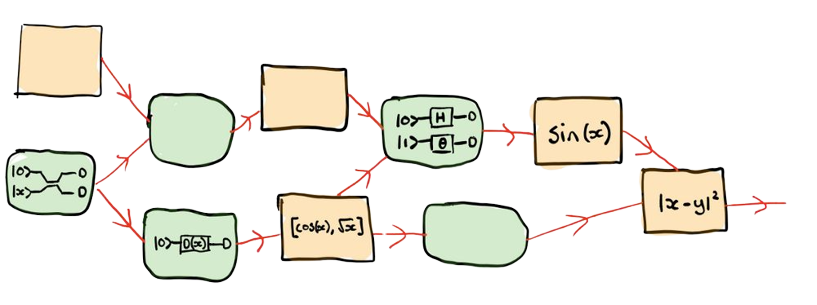
\includegraphics[width=.6\linewidth]{qbackprop}
		\end{center}	
		
		\item specialized, user-friendly, high-performance software (Pennylane, Qiskit, Tensorflow Quantum, ...)
		
		\item 
%		\alert{hybrid} computation
%		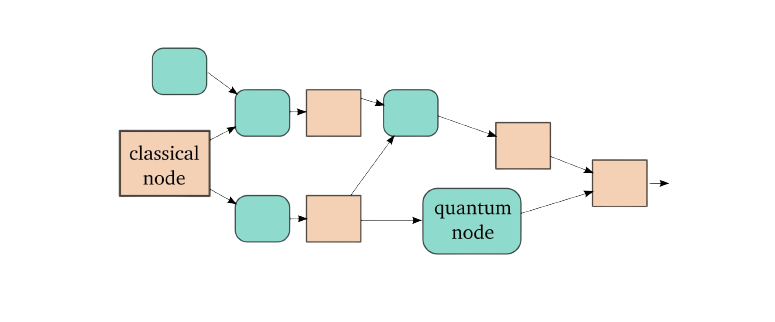
\includegraphics[width=.7\linewidth]{hybrid}
		\begin{minipage}[c]{0.3\textwidth}
			\alert{hybrid} computation
		\end{minipage}
		\begin{minipage}[c]{0.6\textwidth}
			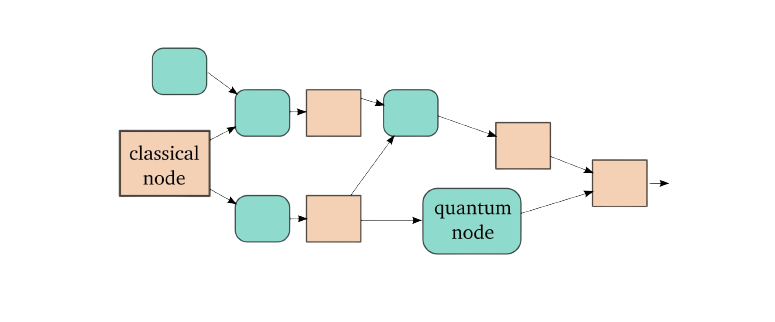
\includegraphics[width=\linewidth]{hybrid}
		\end{minipage}
		
	\end{itemize}
\end{frame}
	% path for images
\graphicspath{{assets/qlearnkit/}}

\section{Qlearnkit}

%% ROBA

\subsection{Quantum Support Vector Machines}

\subsection{Quantum Long-Short Term Memory}
	
	
    %% VA COMMENTATO ANCHE QUESTO !!!
	\begin{frame}{References}
		Some references to showcase [allowframebreaks] \cite{knuth92,ConcreteMath,Simpson,Er01,greenwade93}
	\end{frame}
	
    \graphicspath{{assets/conclusions/}}


\section{Conclusion}
    %%
    \begin{frame}{Summary - Takeaways}
        \begin{itemize}
            \item Quantum computing offers interesting perspectives in several fields (Machine Learning, Cryptography, Quantum Internet, Business, ...)
            \item It's too early to put anything in \alert{production}, but there's a lot of \alert{research} in the field
            \item Quantum computing will be a \alert{parallel} form of computing with classical computing — not a \alert{replacement}
            \item Every business should get prepared in advance for it and its potentially \alert{outbreaking} results
        \end{itemize}        
    \end{frame}

    %%
	\begin{frame}{Summary}
    	All the material used for this presentation is available at the following link:
		
    	\begin{center}
    		\url{https://github.com/mspronesti/talk-qml-amadeus}
    	\end{center}
    	\begin{center}\ccbysa\end{center}
    \end{frame}

       %%
	\begin{frame}{Summary}
    	% Qlearnkit is available at:
    	\begin{minipage}[c]{0.2\textwidth}
    	\centering
			
\includegraphics[width=0.5\linewidth]{gh_logo}
		\end{minipage}
		\begin{minipage}[c]{0.7\textwidth}
    		\url{https://github.com/mspronesti/qlearnkit}
		\end{minipage}
    	
    	
    	% And can be installed with:
    	 \vspace{\abovedisplayskip}
    	\begin{minipage}[c]{0.2\textwidth}
    	\centering
			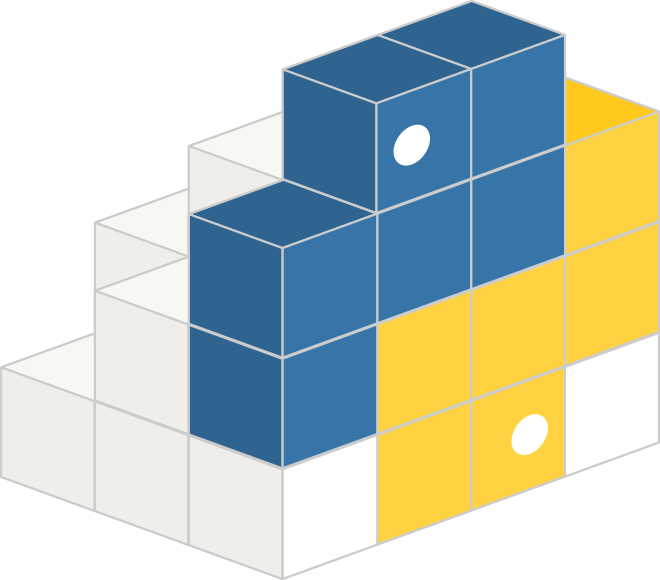
\includegraphics[width=0.5\linewidth]{pypilogo}
		\end{minipage}
		\begin{minipage}[c]{0.7\textwidth}
                \texttt{\$ pip install qlearnkit}
		\end{minipage}
		
    	\begin{center}\ccbysa\end{center}
    \end{frame}
	
	
	%% Questions Slide
	
	\begin{frame}[standout]
		Thanks for your attention!\\
		 Any Question? ~\alert{\faSmileO}~
	\end{frame}
	
	
	\appendix
	
	%% Bibliography
	\begin{frame}[allowframebreaks]{References}
		\bibliography{ref}
		\bibliographystyle{abbrv}
	\end{frame}
	
\end{document}
